

\tikzset{every picture/.style={line width=0.75pt}} %set default line width to 0.75pt        

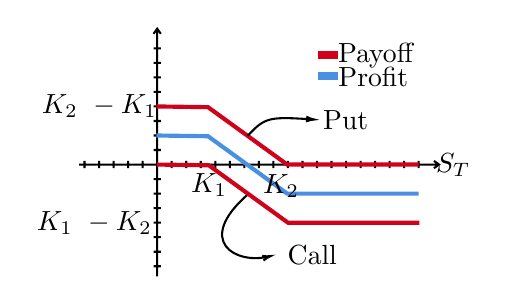
\begin{tikzpicture}[x=0.75pt,y=0.75pt,yscale=-0.35,xscale=0.35]
%uncomment if require: \path (0,363); %set diagram left start at 0, and has height of 363

%Shape: Axis 2D [id:dp5006858190484493] 
\draw  (14,195) -- (509.5,195)(121.5,8) -- (121.5,349) (502.5,190) -- (509.5,195) -- (502.5,200) (116.5,15) -- (121.5,8) -- (126.5,15) (141.5,190) -- (141.5,200)(161.5,190) -- (161.5,200)(181.5,190) -- (181.5,200)(201.5,190) -- (201.5,200)(221.5,190) -- (221.5,200)(241.5,190) -- (241.5,200)(261.5,190) -- (261.5,200)(281.5,190) -- (281.5,200)(301.5,190) -- (301.5,200)(321.5,190) -- (321.5,200)(341.5,190) -- (341.5,200)(361.5,190) -- (361.5,200)(381.5,190) -- (381.5,200)(401.5,190) -- (401.5,200)(421.5,190) -- (421.5,200)(441.5,190) -- (441.5,200)(461.5,190) -- (461.5,200)(481.5,190) -- (481.5,200)(101.5,190) -- (101.5,200)(81.5,190) -- (81.5,200)(61.5,190) -- (61.5,200)(41.5,190) -- (41.5,200)(21.5,190) -- (21.5,200)(116.5,175) -- (126.5,175)(116.5,155) -- (126.5,155)(116.5,135) -- (126.5,135)(116.5,115) -- (126.5,115)(116.5,95) -- (126.5,95)(116.5,75) -- (126.5,75)(116.5,55) -- (126.5,55)(116.5,35) -- (126.5,35)(116.5,215) -- (126.5,215)(116.5,235) -- (126.5,235)(116.5,255) -- (126.5,255)(116.5,275) -- (126.5,275)(116.5,295) -- (126.5,295)(116.5,315) -- (126.5,315)(116.5,335) -- (126.5,335) ;
\draw   ;
%Straight Lines [id:da13258465142858888] 
\draw [color={rgb, 255:red, 208; green, 2; blue, 27 }  ,draw opacity=1 ][line width=1.5]    (120.5,115) -- (191.5,116) -- (300.5,195) -- (481.5,195) ;


%Straight Lines [id:da7932939446362234] 
\draw [color={rgb, 255:red, 208; green, 2; blue, 27 }  ,draw opacity=1 ][line width=3]    (343.5,44) -- (370.5,44) ;


%Straight Lines [id:da14367852228745004] 
\draw [color={rgb, 255:red, 74; green, 144; blue, 226 }  ,draw opacity=1 ][line width=3]    (343.5,73) -- (370.5,73) ;



%Curve Lines [id:da6986177249173428] 
\draw    (246,155.5) .. controls (270.26,129.26) and (276.38,129) .. (335.69,132.88) ;
\draw [shift={(337.5,133)}, rotate = 183.75] [color={rgb, 255:red, 0; green, 0; blue, 0 }  ][line width=0.75]    (10.93,-3.29) .. controls (6.95,-1.4) and (3.31,-0.3) .. (0,0) .. controls (3.31,0.3) and (6.95,1.4) .. (10.93,3.29)   ;

%Curve Lines [id:da16730216097312656] 
\draw    (247,235.5) .. controls (172.25,300.35) and (229.33,333.34) .. (276.09,321.38) ;
\draw [shift={(277.5,321)}, rotate = 524.54] [color={rgb, 255:red, 0; green, 0; blue, 0 }  ][line width=0.75]    (10.93,-3.29) .. controls (6.95,-1.4) and (3.31,-0.3) .. (0,0) .. controls (3.31,0.3) and (6.95,1.4) .. (10.93,3.29)   ;

%Straight Lines [id:da38075245439918526] 
\draw [color={rgb, 255:red, 74; green, 144; blue, 226 }  ,draw opacity=1 ][line width=1.5]    (120.5,155) -- (191.5,156) -- (300.5,235) -- (481.5,235) ;


%Straight Lines [id:da001223510828637031] 
\draw [color={rgb, 255:red, 208; green, 2; blue, 27 }  ,draw opacity=1 ][line width=1.5]    (121.5,195) -- (192.5,196) -- (301.5,275) -- (482.5,275) ;



% Text Node
\draw (529,196) node  [align=left] {$\displaystyle S_{T}$};
% Text Node
\draw (193,223) node   {$K_{1}$};
% Text Node
\draw (422,45) node  [align=left] {Payoff};
% Text Node
\draw (419,74) node  [align=left] {Profit};
% Text Node
\draw (42,115) node   {$K_{2} \ -K_{1}$};
% Text Node
\draw (292,224) node   {$K_{2}$};
% Text Node
\draw (381,134) node  [align=left] {Put};
% Text Node
\draw (335,320) node  [align=left] {Call};
% Text Node
\draw (35,275) node   {$K_{1} \ -K_{2}$};


\end{tikzpicture}

